\chapter{Implementation of Lane detection algorithm on UGV using Raspberry Pi.}
\section{Introduction}
\par Lane detection is a primary step for vehicles to be autonomous. For self-driving cars, lane detection helps to navigate vehicles in predefined lanes. There are many algorithms which accomplish this task efficiently. It also helps the visual perception of vehicles in real-time navigation.
I have used the simplest approach ‘Hough Transform’ algorithm for lane detection.  
The entire project is divided in 3 parts:
\begin{enumerate}
    \item Gaussian Blur + Canny Edge Detection
    \item Hough Transform
    \item Displaying the lines + Thresholding 
\end{enumerate}

\section{Software and Hardware Requirements}
\subsection{Libraries to be installed}
\begin{itemize}
    \item Numpy (used for performing mathematical computations)
    \item OpenCV (used to make computer vision applications)
    \item Matplotlib (used to visualize the images)
    \item Hough Transform Algorithm
    \item Raspberry Pi 
    \item UGV kit (chassis, motors, motor driver IC, jumper wires)
    \item Pi camera 
\end{itemize}

\subsection{Hough Transform}
\par In the Cartesian plane (x and y-axis), lines are defined by the formula y=mx+b, where x and y correspond to a specific point on that line and m and b correspond to the slope and y-intercept.
\begin{figure}[h!]
\centering
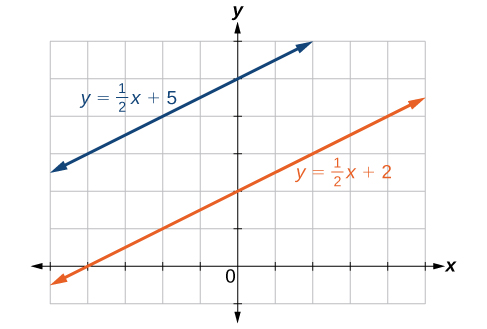
\includegraphics[width=10cm]{./Figures/hough_transform.jpeg}
\caption{Lines in Cartesian Coordinate Space}
\label{Lines_in_Cartesian_Coordinate_Space}
\end{figure}
\par A regular line plotted in the Cartesian plane has 2 parameters (m and b), meaning a line is defined by these values. Also, it is important to note that lines in the Cartesian plane are plotted as a function of their x and y values, meaning that we are displaying the line with respect to how many (x, y) pairs make up this specific line (there is an infinite amount of x, y pairs that makeup any line, hence the reason why lines stretch to infinity).
However, it is possible to plot lines as a function of its m and b values. This is done in a plane called Hough Space. To understand the Hough Transform algorithm, we need to understand how Hough Space works.
\subsubsection{Explanation of Hough Space}
\begin{itemize}
    \item Points on the Cartesian plane turn into lines in Hough Space
    \item Lines in the Cartesian plane turn into points in Hough Space
    \item We can find the line of best fit of two points in Cartesian space by finding the m and b coordinates of the POI (point of intersection) of the two lines that correspond with these points in Hough Space, then forming a line based on these m and b values.
\end{itemize}

\begin{figure}[h!]
\centering
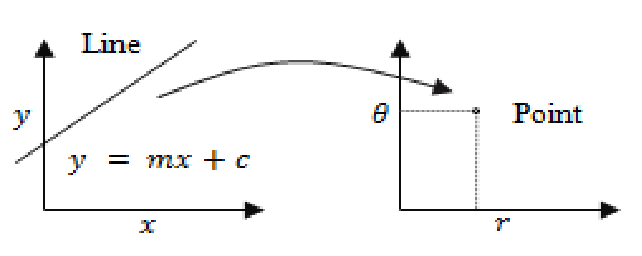
\includegraphics[width=8cm]{./Figures/graph_lane_detection.png}
\caption{Explanation of Hough Space}
\label{Explanation_of_Hough_Space}
\end{figure}

\par A line is basically an infinitely long grouping of points arranged orderly one after the other. Since on the Cartesian plane, we’re plotting lines as a function of x and y, lines are displayed as infinitely long because there is an infinite number of (x, y) pairs that make up this line.
Now in Hough Space, we’re plotting lines as a function of their m and b values. And since each line has its only one m and b value per Cartesian line, this line would be represented as a point. 

\section{Lane detection flow diagram}
\begin{figure}[h!]
\centering
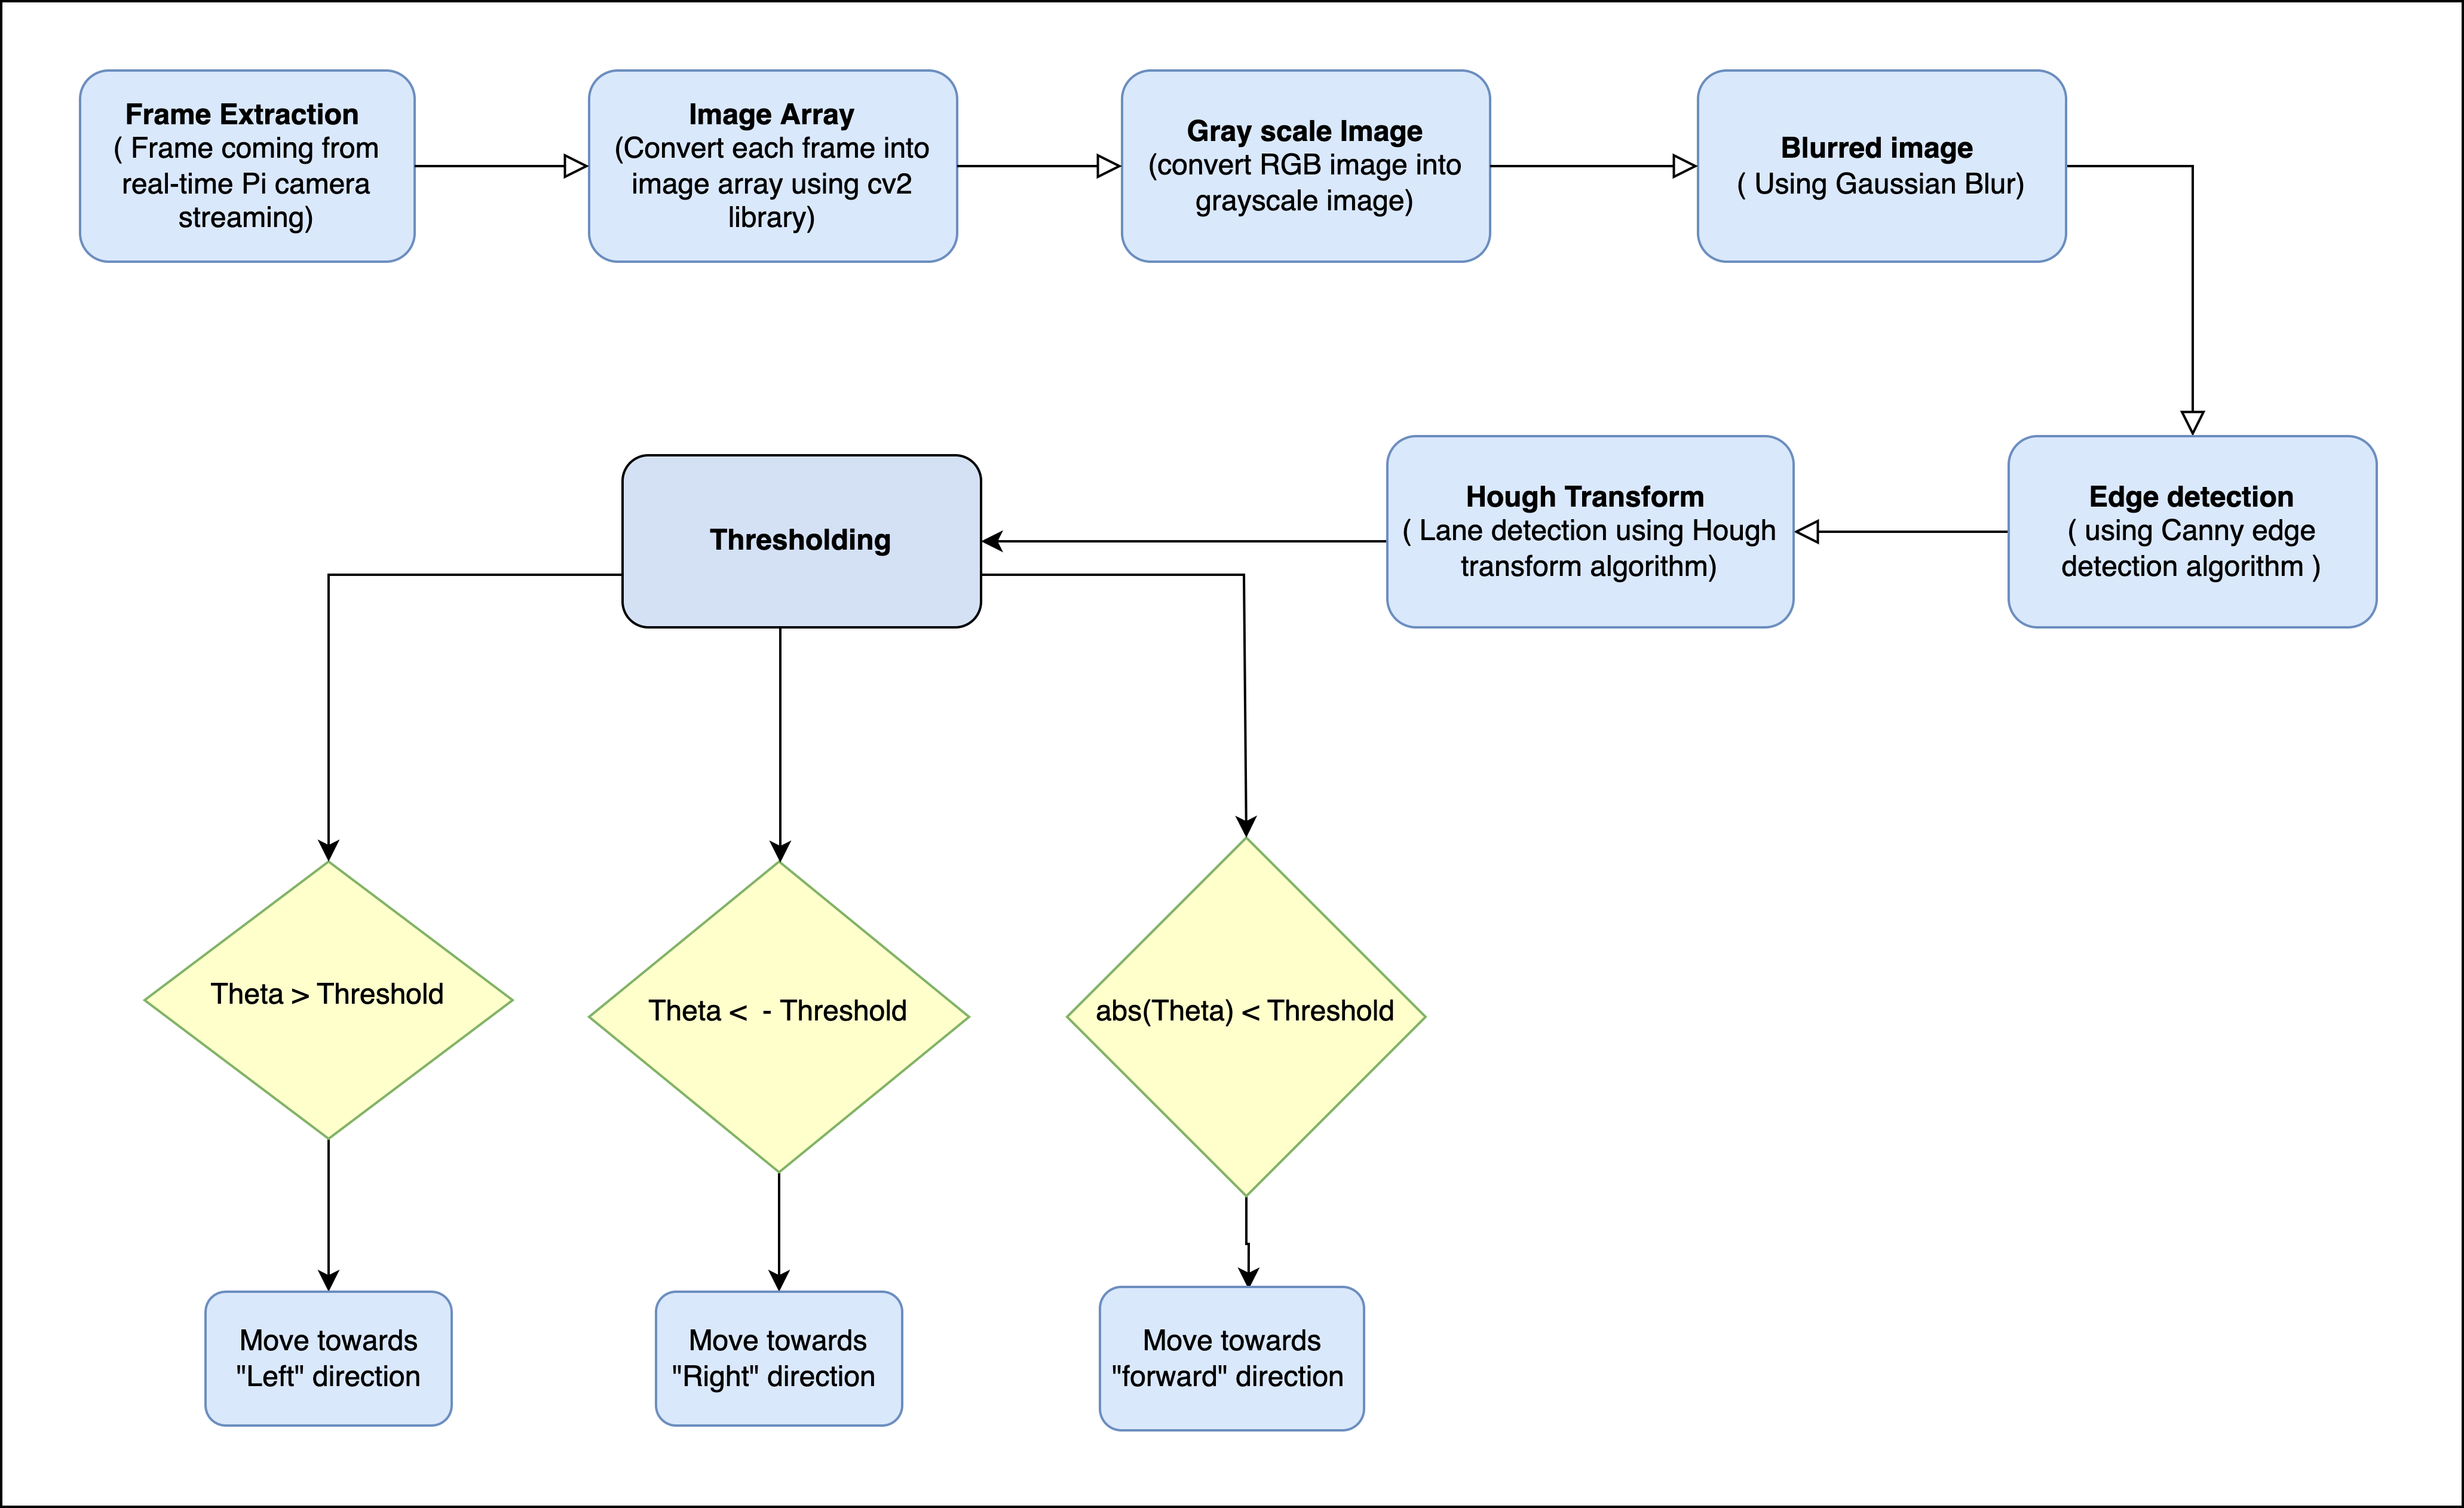
\includegraphics[width=\columnwidth]{./Figures/lane_detection.png}
\caption{Flow diagram for Lane detection}
\label{Flow_diagram_for_Lane_detection}
\end{figure}

\begin{figure}[h!]
\centering
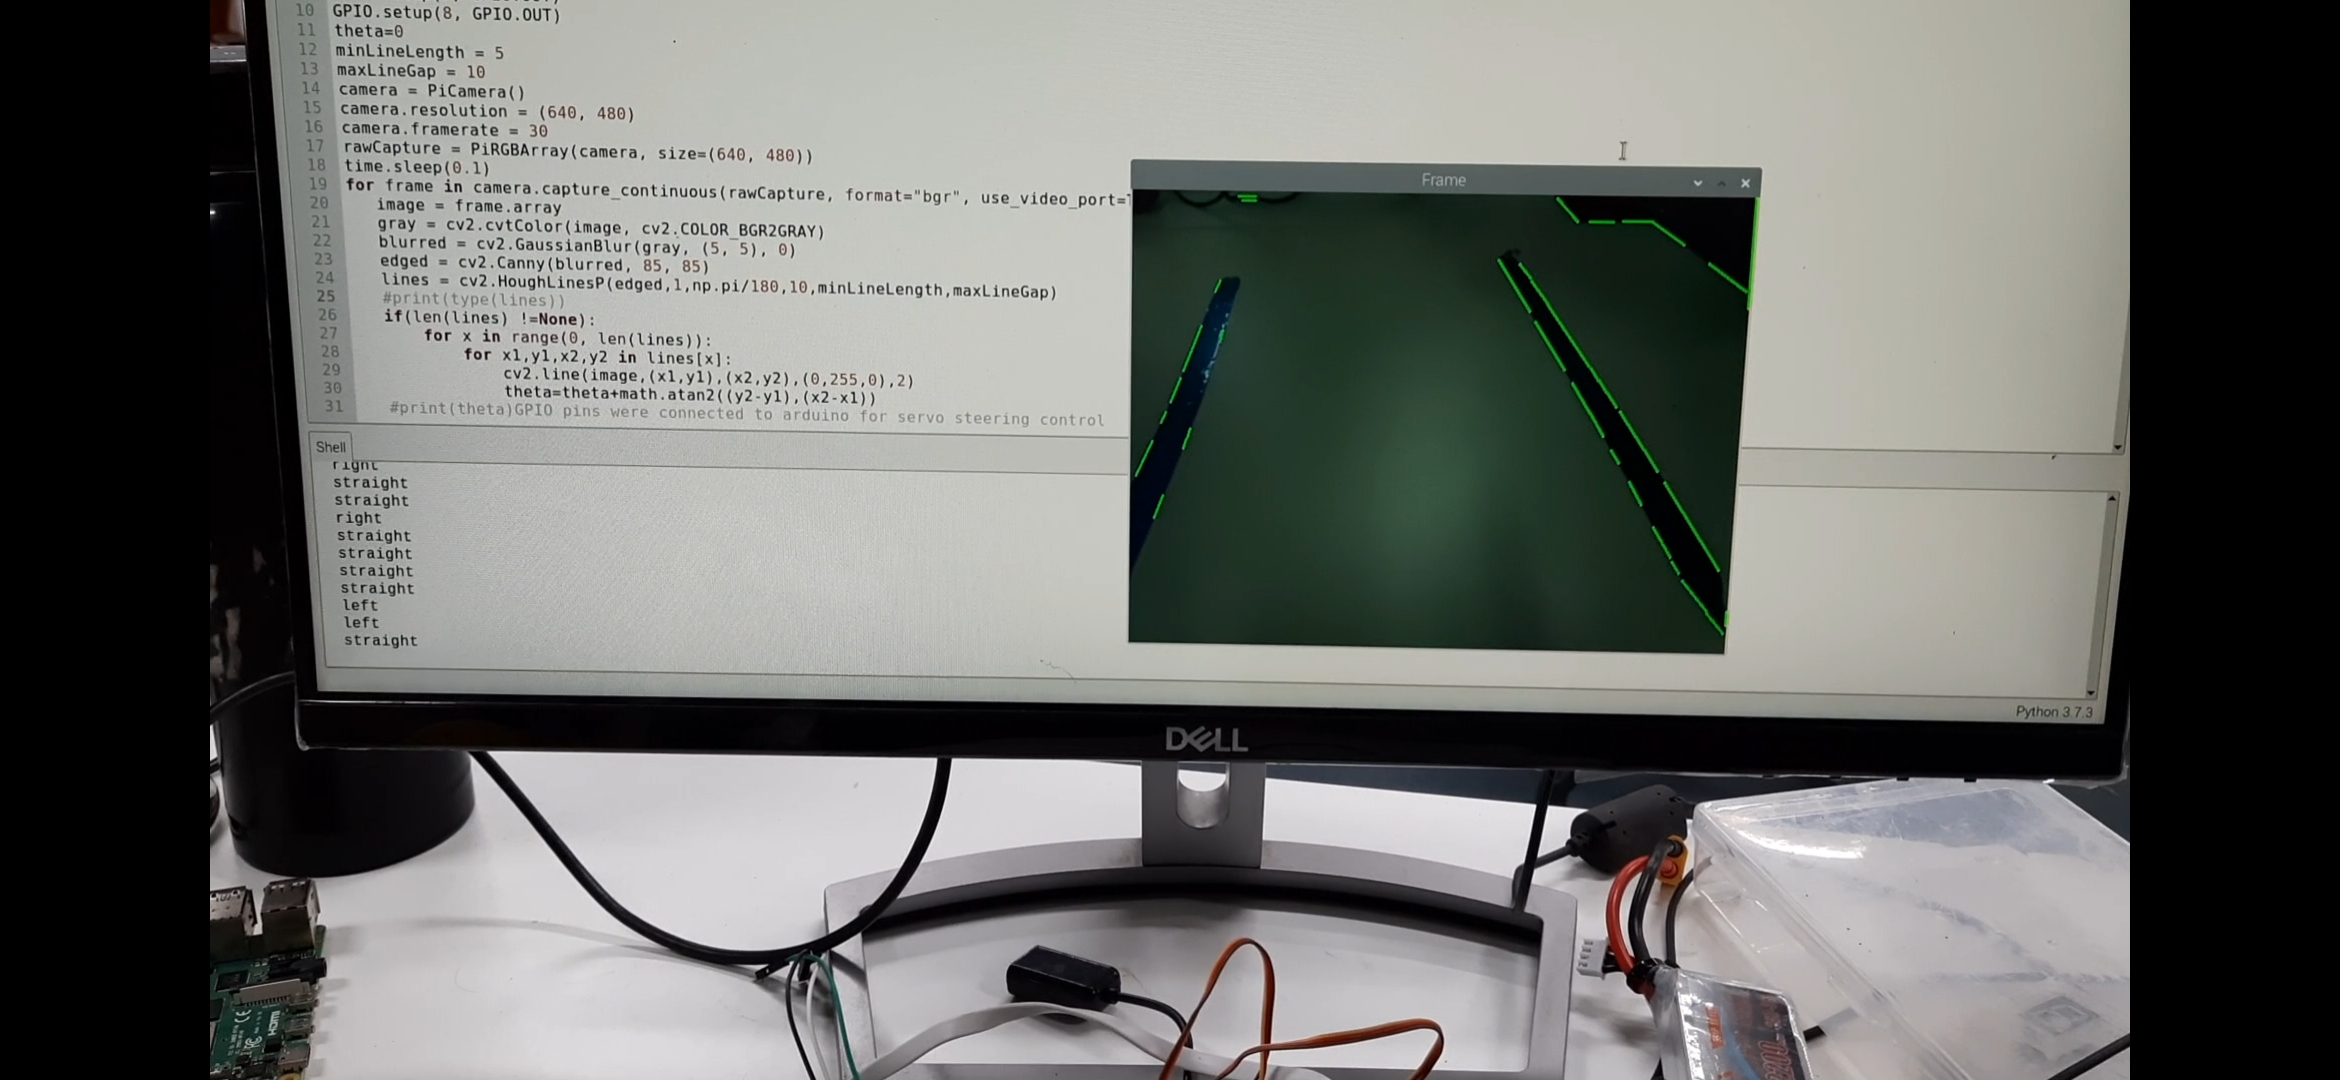
\includegraphics[width=\columnwidth]{./Figures/actual_lane_detection.jpg}
\caption{A glimpse of lane detection in lab}
\label{actual_lane_detection}
\end{figure}

\subsection{Steps}
\begin{itemize}
    \item Frame extracted from continuous stream of camera on Pi.
    \item Each frame is converted into an image array by using openCV library.
    \item Now, the image array is converted into a gray-scale image.This helps by increasing the contrast of the colours, making it easier to identify changes in pixel intensity.
    \item Using a Gaussian filter, we try to blur the image in order to reduce the noise in images.We do this because the gradients in Canny edge detection (in further step) are really sensitive to noise, so we want to eliminate the most noise possible.
    \item Canny edge detection detects the edges present in images. It calculates the change of pixel intensity (change in brightness) in a certain section in an image. 
    \item Now, we apply Hough transform on post canny edge detection images. This turns edges into lines that can be seen in images as detected lanes.
    \item After detection of lines, I have used thresholding techniques. The ‘Theta’ (averaging of lines) is used to give command to motor driver IC to maintain the vehicle in lane ( refer flow diagram for thresholding conditions).
    \item A continuous left, right or straight command is coming as output ( for user reference) as per real-time scenarios. The vehicle takes those commands to maintain its navigation within lanes.
\end{itemize}



\subsubsection{All files, codes and resources related to Lane detection can be found at below GitHub link} 
\begin{tcolorbox}
        \url{https://github.com/Abhishek-IITH/Lane-Detection-Project.git}
\end{tcolorbox}